\documentclass{article}
\usepackage{doc}

\begin{document}

% 标题
\title{存储引擎模块}
\maketitle

\begin{abstract}
    本文描述存储引擎模块的设计与实现
\end{abstract}

\tableofcontents
\vskip\baselineskip

关系数据库的存储引擎一般包括三个部分：底层存储布局、索引结构、缓冲管理。waterfall项目中，存储引擎代码放在waterfall/storage目录下。

\section{存储布局}

底层存储布局主要处理记录如何摆放在文件中，主要内容包括：功能的段式管理、页面格式、记录格式、元数据管理等。下面从小到大描述存储布局的设计。

\subsection{record}

逻辑上的关系由一行一行数据组成，这是关系数据库的视角。现代kv存储引擎则拆解得更细，key-value对是最小的存储单元。

会话代理用户执行SQL指令，它操纵的是元组tuple，元组用vector来表示。元组落到底层存储上，表示为记录record。由于数据库中元组的字段数目不固定，类型不固定，所以一般记录具有一定的自描述特性，这导致记录一般会带有一定格式。

\begin{figure}[H]
    \centering
    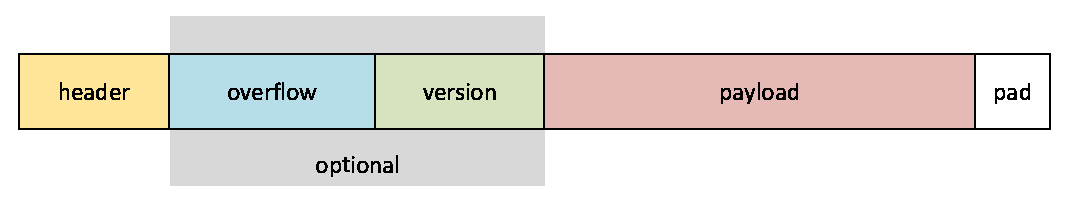
\includegraphics[width=\linewidth]{img/storage/s-record.eps}
    \caption{记录格式}\label{fig:s-record}
\end{figure}

\figurename\ref{fig:s-record}是记录的整体格式，首先是定长2B的记录头，描述记录类型。然后是可选的定长部分，overflow和version。记录可能比较大，当超过页面一半是，定义为溢出记录，这部分表达为一个rid，定长6B。version用于支持mvcc，定长8B，没有采用整型压缩方式，主要为了快速检查版本号。

记录要按照8B对齐，最后会有一个padding字节，填充到8B对齐。这部分不在记录中管理，这是在页面分配的时候需要考虑。

\begin{figure}[H]
    \centering
    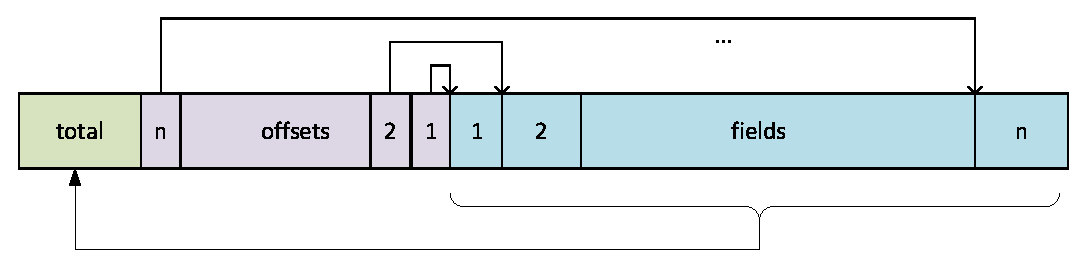
\includegraphics[width=\linewidth]{img/storage/s-payload.eps}
    \caption{payload}\label{fig:s-payload}
\end{figure}

记录载荷的格式如\figurename\ref{fig:s-payload}所示，主要包括三部分：字段长度、偏移量序列、字段序列。字段长度位于payload头部，是第3部分所有字段长度的总和，采用uleb128编码，用于压缩字段长度。第3部分是字段序列，每个字段顺序摆放在这部分中。

偏移量序列是所有字段的倒排序列，第1个偏移量指向最后一个字段，如此类推，最后一个偏移量指向第1个字段，最后一个偏移量为0。所有偏移量俊采用uleb128压缩格式。

payload的设计主要利用了倒排偏移量单调递减的特性，最后一个偏移量一定为0。实际上这个假设并不总是成立，它要求：
\begin{itemize}
    \item 元组不能为空；
    \item 并且第一个字段不能为空；
\end{itemize}
这样一来，这个记录格式的应用就会受限，可以考虑向innodb的聚集存储靠齐。

\subsubsection{TODO}

\begin{itemize}
    \item 实现overflow记录的存储方案。目前代码中，虽然在格式上定义了溢出格式，但并未实现对溢出的支持，设计溢出记录的存储方案。
    \item 实现version记录的存储方案。为支持mvcc，每条记录都会带一个版本号。PostgreSQL的记录采用堆模型，记录可能放在非临近页面，所以在设计上使用ctid指向新记录位置，形成一个版本链。结合课程事务部分的内容，设计一个版本链的存储方案。
\end{itemize}

\subsection{page}

大多数传统关系数据库都采用分页方式存储记录，页面固定大小，以方便缓冲层的设计。会话操作的是元组，事务管理的是元组，但是存储是按照页面为单位进行，系统恢复需要着重关注页面。

\begin{figure}[H]
    \centering
    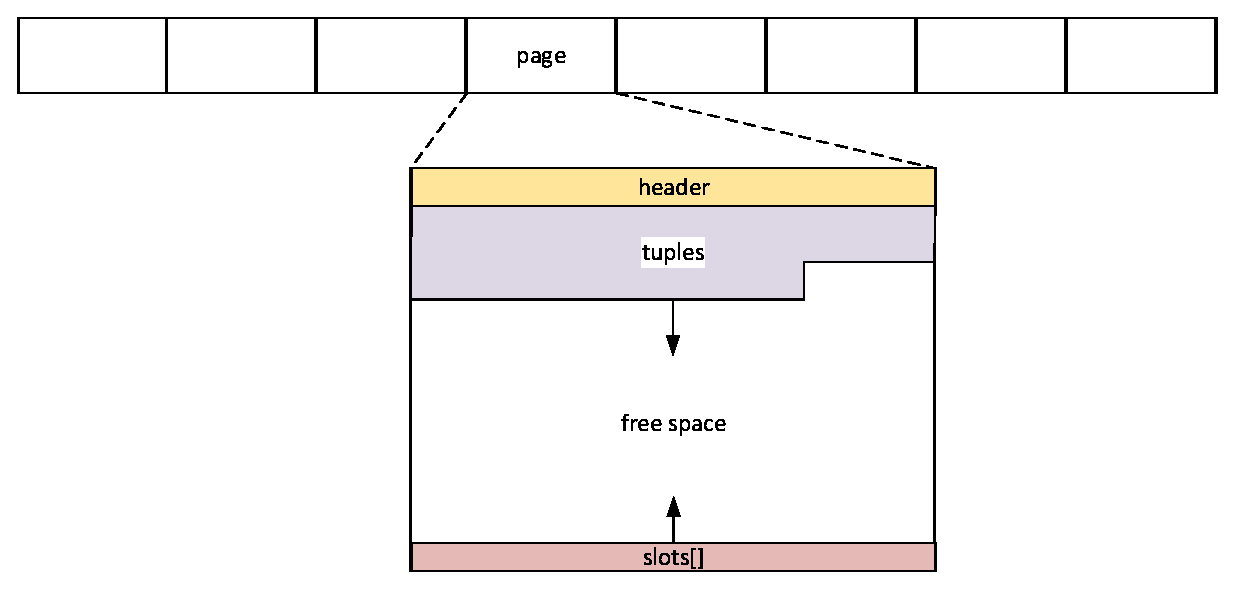
\includegraphics[width=\linewidth]{img/storage/s-page.eps}
    \caption{页面格式}\label{fig:s-page}
\end{figure}

页面也带有格式，如\figurename\ref{fig:s-page}所示。页面的头部是header，包括页面类型、页面LSN等信息、CRC校验、空闲空间大小与指针、记录数目等信息。然后是记录区域，接着是空闲区域，最后是slots[]数组。

由于记录数目会增加，slots[]数组也会增长，空间上从两侧挤压空闲空间。需要说明的是，页面上的可用空间一般是大于等于空闲空间大小，因为被删除的记录只是被标记为tomstone，并没有回收。

\subsubsection*{clustered页面}

页面分为几种类型，一种是聚集页面，用于聚集存储。这类页面中，slots[]数组会按照key排列。slots[]数组里保存的是记录在页面内的偏移量，访问key需要打开页面内的记录，然后找到key。

聚集存储一般会和btree索引一起保存，btree是主索引，聚集页面看成btree的叶子节点。聚集存储中，记录按照key访问，record\_id在聚集存储里没用。同时，辅助索引会over在主索引上，辅助键输出的是主键，然后再利用主键访问记录。

聚集存储利好查询，扫描性能好，同时更新记录，也不用去修改辅助索引。

\subsubsection*{heap页面}

heap页面是一种非聚集存储页面，记录按照插入顺序存储，slots[]数组按照插入顺序排列。在堆模型中，要访问一条记录，需要通过record\_id，record\_id包含页面id和记录的偏移量。

注意，record\_id并不是记录在页面内的偏移量，而是指slots[]数组的下标。因为记录可能被删除，被删除记录的空间要回收，需要在页面内部移动记录，所以record\_id不能指向记录在页面内的偏移量，而是通过slots[]间接指向记录。

在waterfall工程中，heap页面也是有用的。虽然采用聚集存储，但版本一多，页面内容纳的差异记录会减少。大多数应用都是访问最新版本，将最新版本放在聚集页面内有助于提升性能，而老的记录版本则可以放在heap页面中。heap页面的另一个用法是保存元数据，因为这些数据保存在页面内一般不会删除。

\subsubsection{TODO}

\begin{itemize}
    \item 实现clustered页面
    \item 实现heap页面
\end{itemize}

\subsection{segment}

页面用于存储记录，段用于管理多个页面，将多个同功能页面聚集成段。例如，数据段管理所有聚集页面和btree索引页面，空闲段管理所有空闲页面，版本段管理所有老版本记录页面，undo段管理所有checkpoint之后改变的页面。

段的管理使用bitmap，每个页面对应于一个bit，bit为1表示页面在段中，bit为0表示页面不在段中。考虑到随着文件增加，这个bitmap会增长，所以采用roaring\cite{GitHubRo54:online}压缩格式保存，可以直接在fedora上安装这个包。

段的管理信息放在superblock内，superblock是文件的第1/2个页面，用于存储文件的元数据，例如段信息、记录数目等。superblock采用双缓冲策略，即superblock有两个版本，一个是当前版本，一个是备份版本。当superblock需要更新时，先将更新写入备份版本，然后将备份版本切换为当前版本。

\subsubsection{TODO}

\begin{itemize}
    \item 实现superblock双缓冲策略
    \item 实现段的管理操作，例如添加、删除、查询页面是否在段中等
\end{itemize}

\begin{figure}[H]
    \centering
    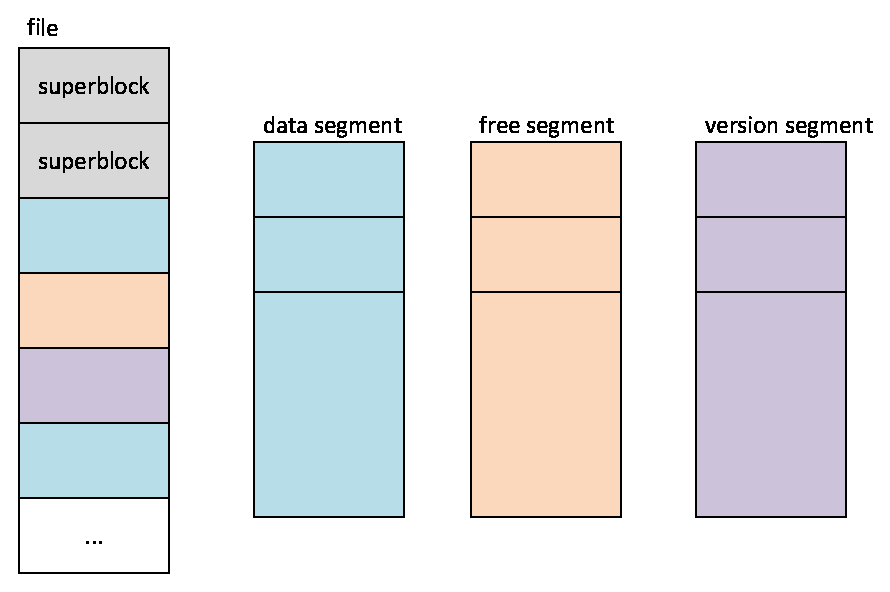
\includegraphics[width=\linewidth]{img/storage/s-segment.eps}
    \caption{功能段}\label{fig:s-segment}
\end{figure}

\section{btree索引}

btree的结构如\figurename\ref{fig:s-btree}所示。btree是一种平衡多叉树，叶子节点、内部节点、根节点大小相同，结构类似，非常适合HDD这样的存储介质保存。

btree的节点布局与\figurename\ref{fig:s-page}相同，这便于缓冲层管理。btree中，每条记录一般就是<key, pos>对，记录中只有两个字段，key是键值，pos是记录在页面内的偏移量。<key, pos>的条目在页面尾部slots[]按照key顺序排列，采用二分查找。

\begin{figure}[H]
    \centering
    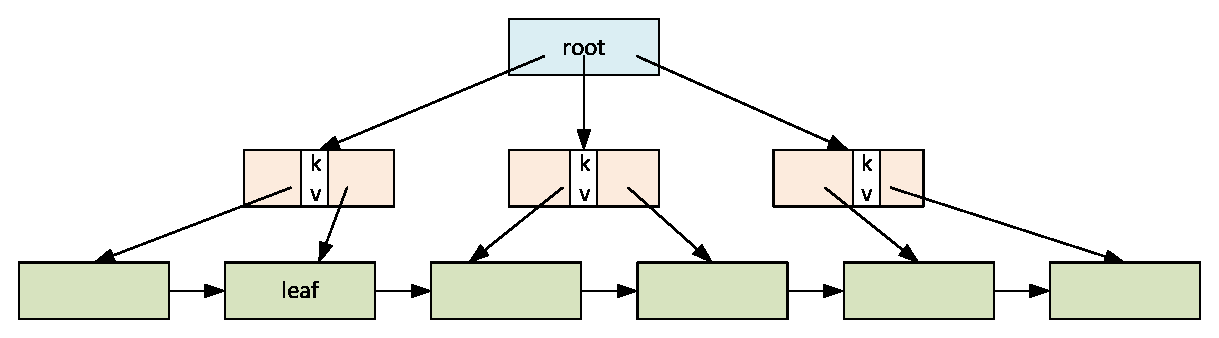
\includegraphics[width=\linewidth]{img/storage/s-btree.eps}
    \caption{btree结构}\label{fig:s-btree}
\end{figure}

<key, pos>构成了btree的key和右指针，btree根节点和内部节点的最左指针，借用页面头部的header的next指针。数据页面看成btree的叶子节点，btree主索引与数据页面一起存放在一个文件中。

btree的主要功能是：查找、插入、删除。查找需要返回完整的搜索路径，以供后续插入和删除操作使用。插入可能会导致节点分裂，分裂可能递归向上，需要完整处理。删除的情况更复杂些，当节点容量减小，需要向兄弟节点借记录，进一步可能需要合并兄弟节点，合并还可能递归向上。

另外，插入、删除动作向上递归，可能会导致加latch出问题，因为latch一般总是一个方向加锁，向上递归时，可能会导致死锁。在处理插入、删除时，需要在新轮里从上向下处理，避免死锁。

辅助索引里，会出现重复项，一个key可能对应多个指针。采用记录可以保存多个指针，也就是说，在btree中，以<key, pos1, pos2, ...>形式处理重复项。

\subsubsection{TODO}

\begin{itemize}
    \item 实现btree索引的查找、插入、删除操作
    \item 实现一个内存版本btree，借助与缓冲层的大容量页面，实现单轮关系算子的连接、差等算法。
\end{itemize}

\section{缓冲管理}

缓冲层主要用于管理页面，缓冲层采用队列形式管理页面，包含：lru队列、空闲队列、脏页队列、fix队列等。每个页面关联一个latch，latch用于保护页面的并发访问。页面通过<fd, page\_id>唯一标识，fd表示文件描述符。整体上，缓冲管理是一个多维结构，每个维度负责不同的功能。

\begin{figure}[H]
    \centering
    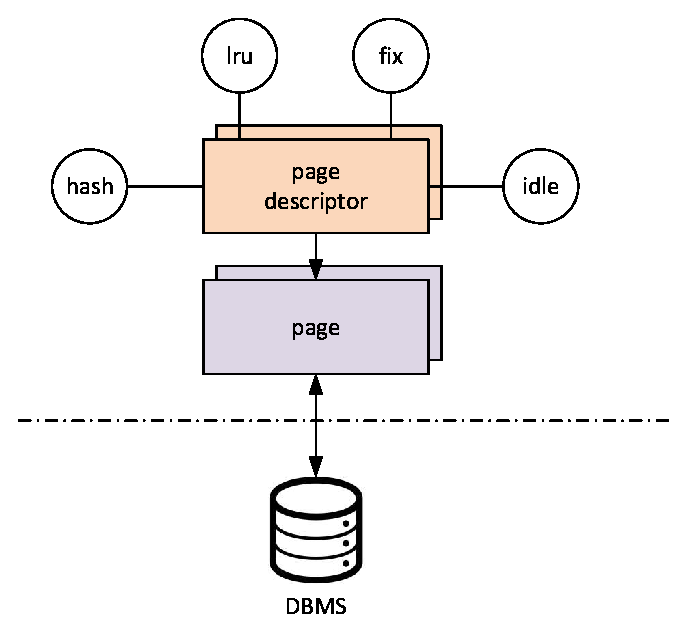
\includegraphics[width=0.6\linewidth]{img/storage/s-buffer.eps}
    \caption{缓冲层结构}\label{fig:s-buffer}
\end{figure}

\subsubsection*{hash表}

以<fd, page\_id>作为key，指向一个页面描述结构，描述结构包括latch、页面指针等。设置hash表是为了快速找到对应的页面，而不是从硬盘上读出。

\subsubsection*{lru队列}

lru队列是最近最少访问页面队列，一个最近读写的页面被移动到队头。设置lru队列的目的是，是为了swap，当页面不敷使用，需要淘汰最近最少访问的页面。

\subsubsection*{idle队列}

空闲队列管理为使用内存页面。

\subsubsection*{fix队列}

fix队列用于管理固定页面，这些页面被固定在内存中，不会被swap出去。fix上的有些页面，并没有对应的<fd, page\_id>，这些页面用于保存内存btree节点。

缓冲的页面管理还有些需要注意的地方：
\begin{itemize}
    \item dirty标志位，用于标志页面是否被修改。swap时，dirty页面被回写，clean页面进入idle队列重新分配。
    \item checkpoint，要将dirty页面回写，这个开销比较大，可以拉长checkpoint过程，避免对系统冲击过大。
    \item 文件采用异步io方式读写，避免阻塞线程。
    \item 不得采用mmap方式打开文件，避免mmap页面被操作系统交换到虚拟内存上。
    \item 直接用mmap申请buffer页面，这些内存直接固定在物理内存中，不允许交换到虚拟内存。
\end{itemize}

\subsubsection{TODO}

\begin{itemize}
    \item 实现buffer管理层
\end{itemize}

% 参考文献
\printbibliography

% 附录
\appendix

\end{document}